%doc: 2a tramesa revista/revista_6/6_dibuix_del_natural/parmera.doc
\newpage
\begin{news}
{2} %columnes
{Els Alumnes de 6è dibuixem la palmera del pati de sorra}
%index: La palmera del pati
{Fa unes setmanes, els alumnes de sisè de primària vam sortir al pati de sorra de l’escola per fer un dibuix del natural}
{Primaria}
{37}


Havíem de dibuixar la palmera del pati de sorra amb el màxim de detalls possibles. Per això ens hi havíem de fixar molt bé.

Primer la vam dibuixar en un full amb el llapis.

Després vam tornar a la classe i ens van donar un altre full.

En aquest segon full havíem de dibuixar la palmera una segona vegada, però en aquest cas no podíem utilitzar el llapis per res. Havíem de dibuixar directament  amb un punta fina, així que, si ens equivocàvem,  no hi havia forma d’arreglar-ho. Per sort,  no ens vam equivocar gaire.

\end{news}

\begin{news}
{3} %columnes
{}
{Aquí teniu una petita mostra del que vam fer: Marc Gómez, Laura Gómez i Daniel Sánchez}
{}
{37}


\noindent\fbox{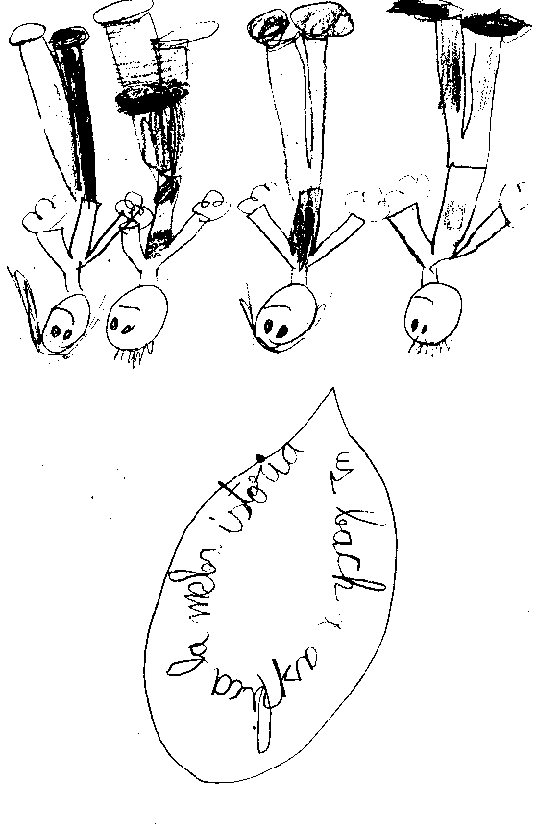
\includegraphics[width=5cm,keepaspectratio,angle=180]{primaria/img/palmera003103.jpg}}

\noindent\fbox{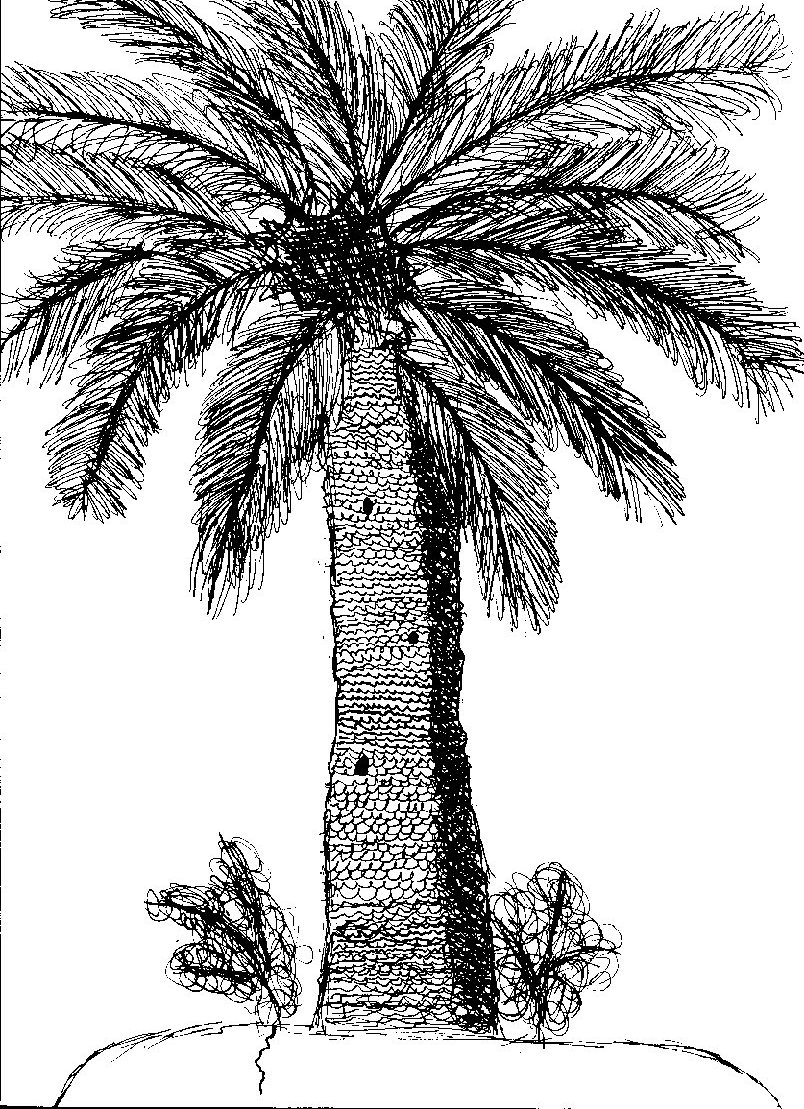
\includegraphics[width=5cm,keepaspectratio]{primaria/img/palmera001100.jpg}}

\noindent\fbox{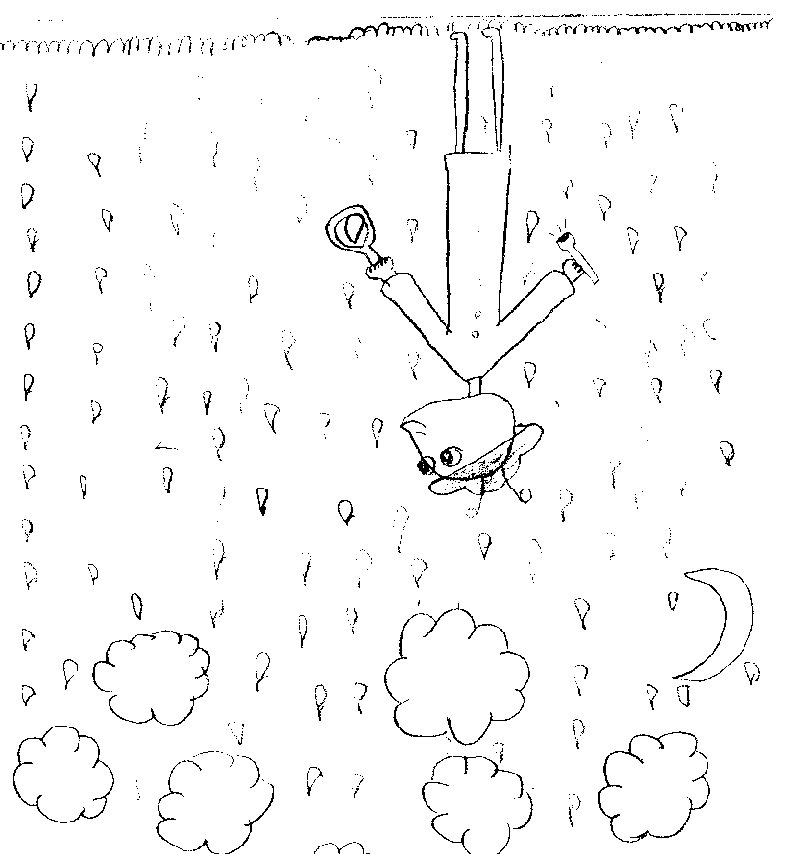
\includegraphics[width=5cm,keepaspectratio,angle=180]{primaria/img/palmera003104.jpg}}

\noindent\fbox{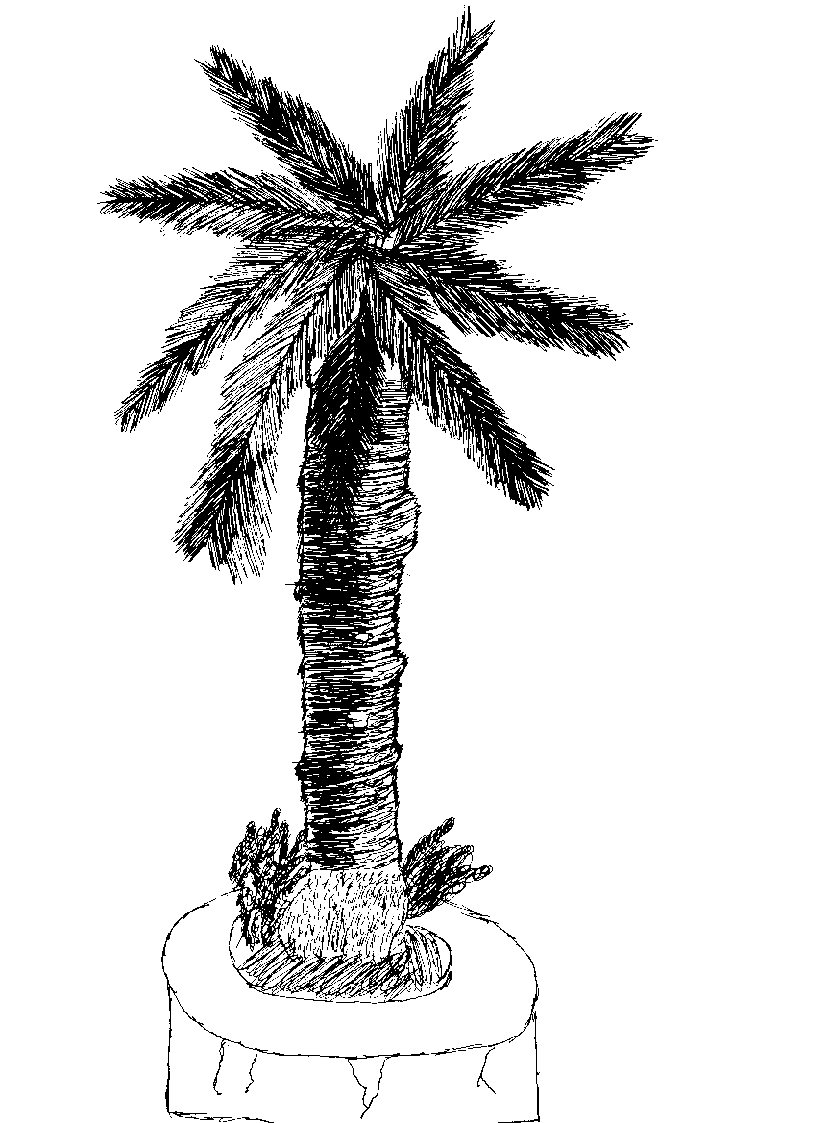
\includegraphics[width=5cm,keepaspectratio]{primaria/img/palmera002101.jpg}}


\noindent\fbox{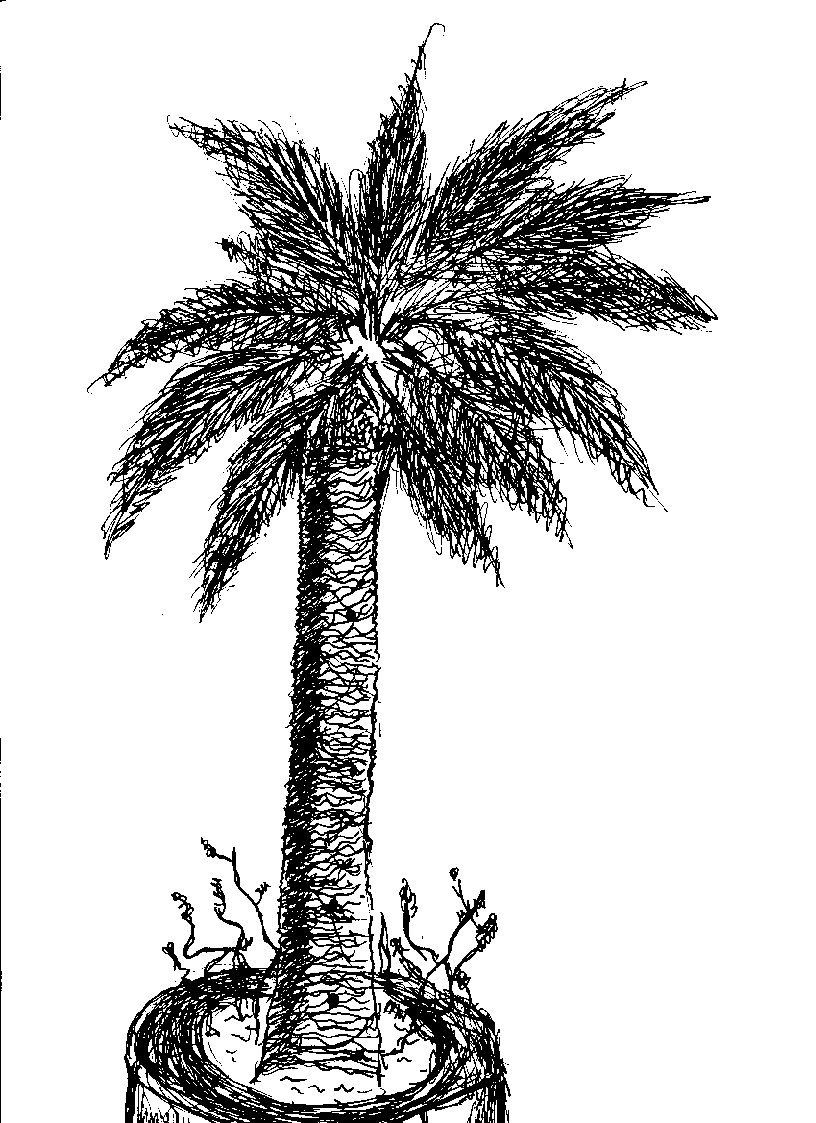
\includegraphics[width=5cm,keepaspectratio]{primaria/img/palmera003102.jpg}}




\end{news}

\begin{news}
{2}
{}
{}
{}
{}

\noindent\fbox{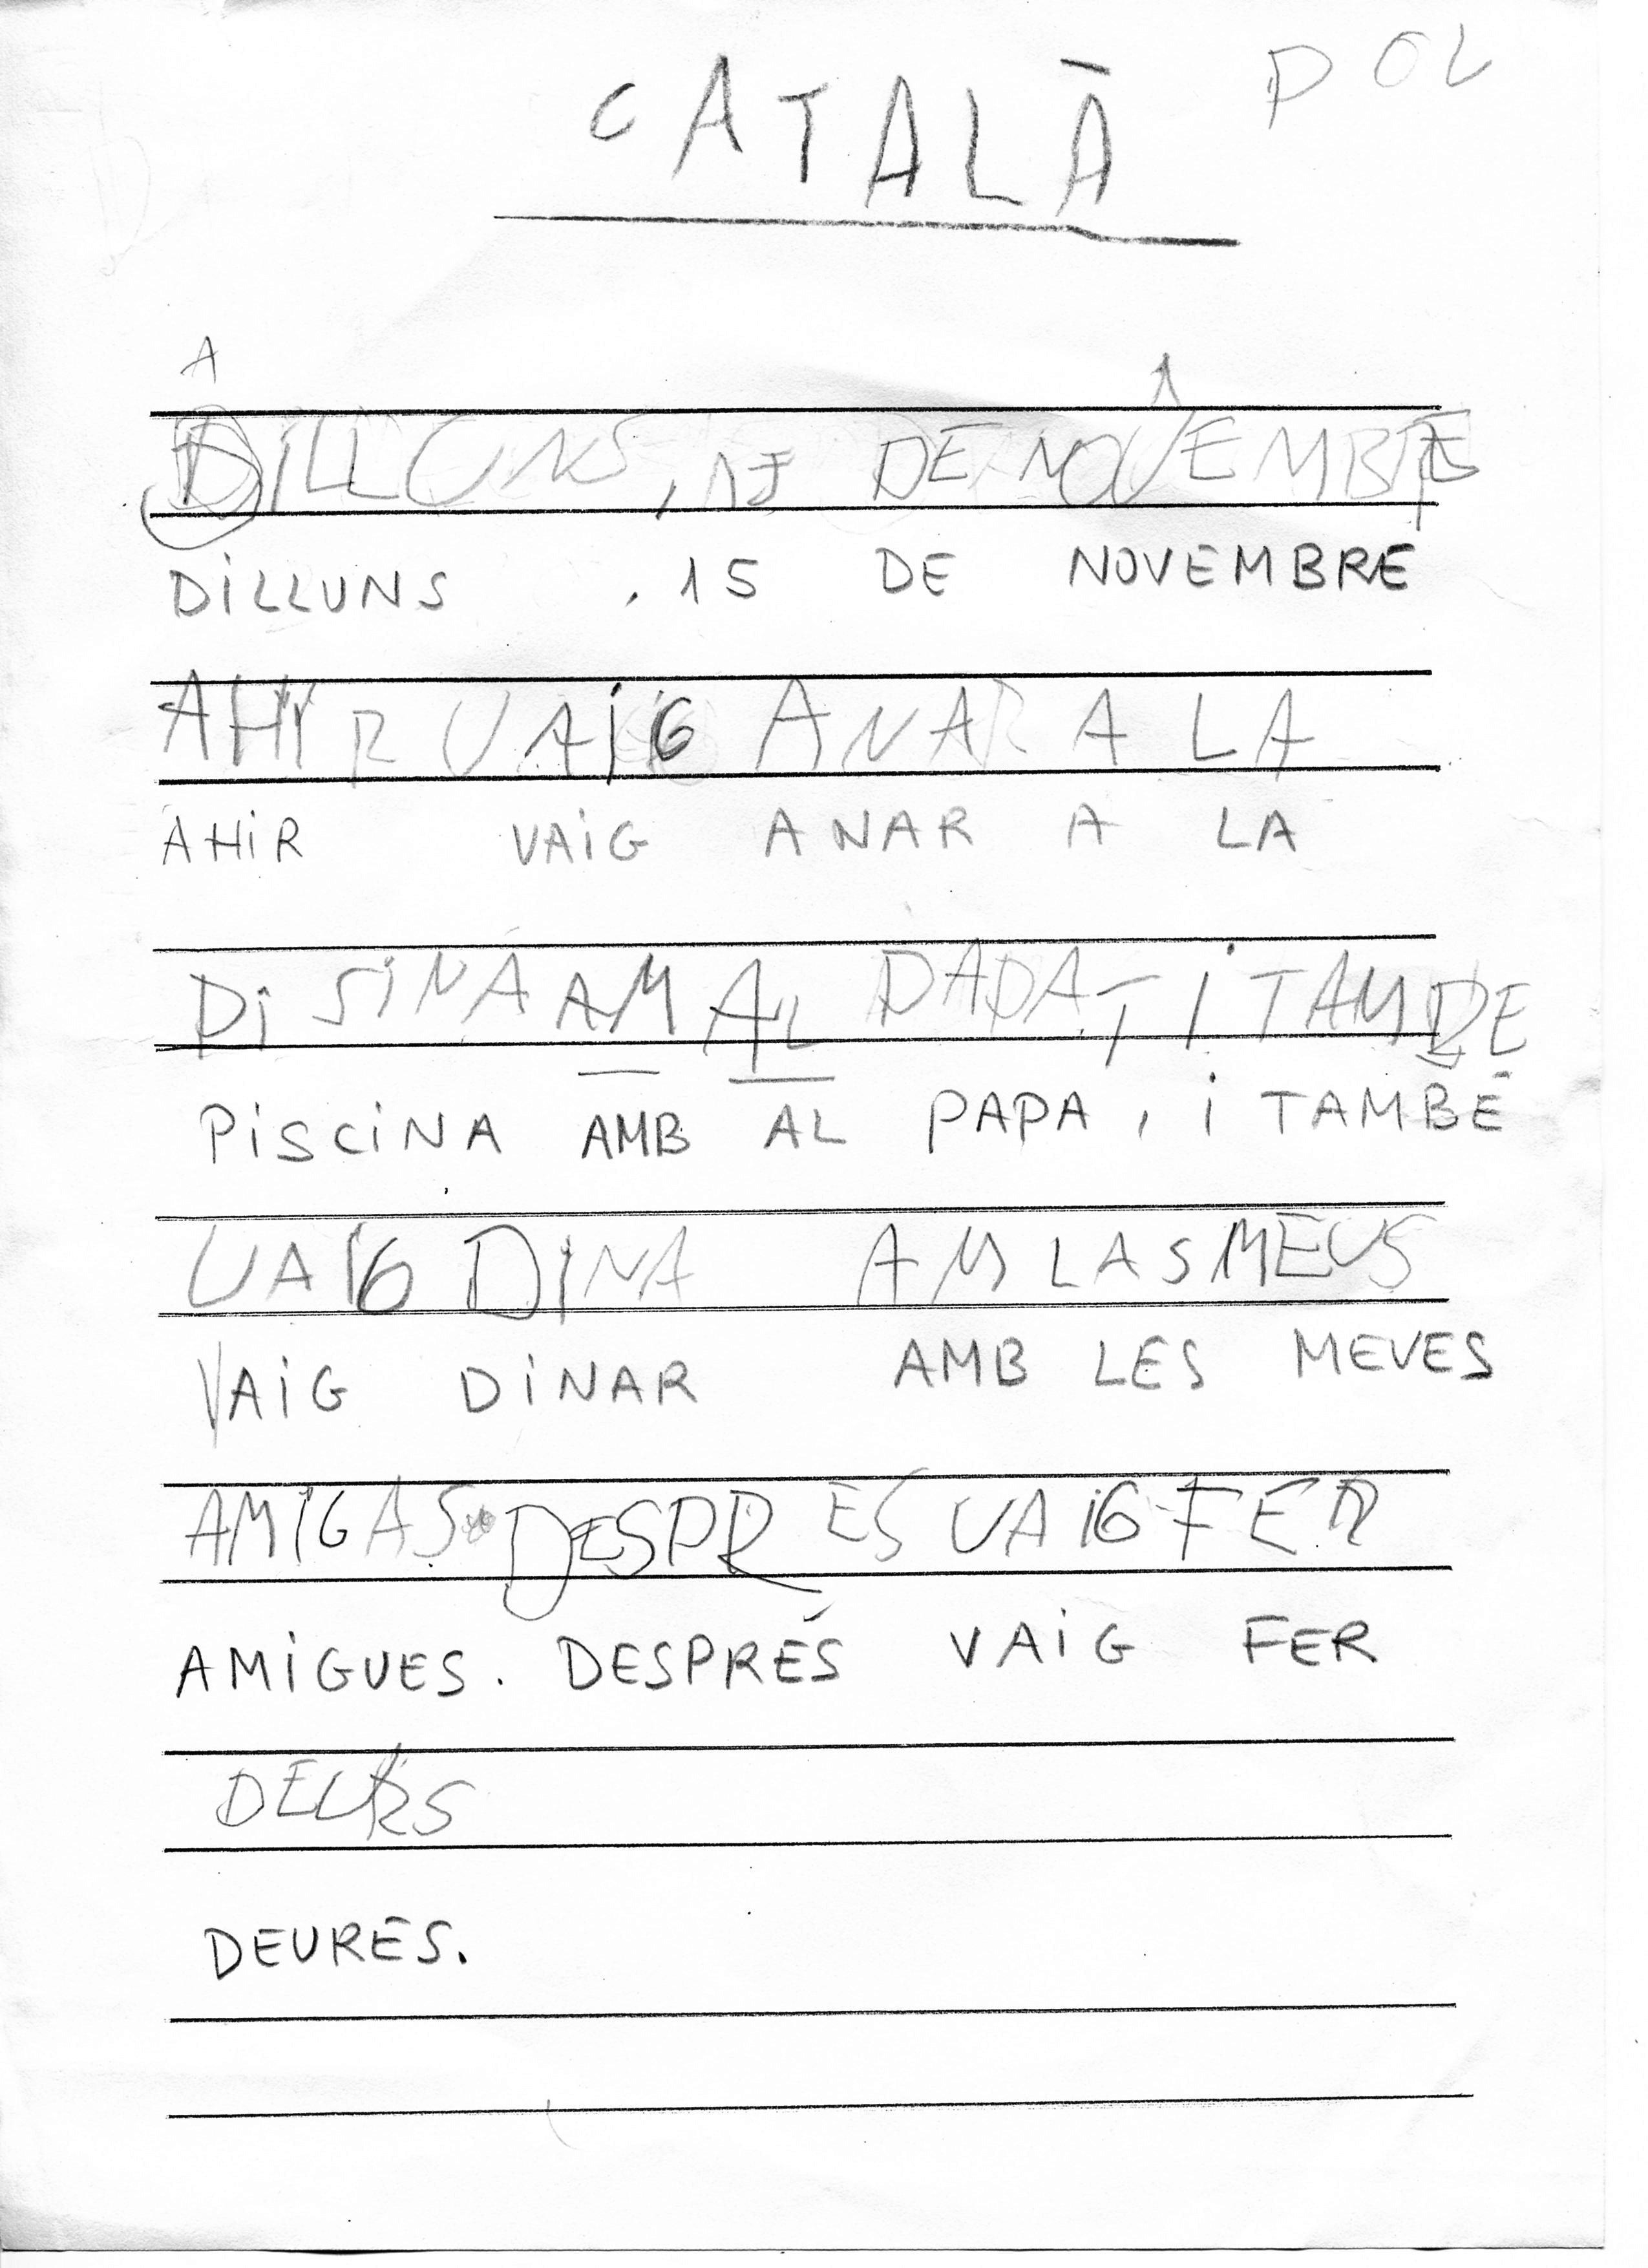
\includegraphics[width=8cm,keepaspectratio]{primaria/img/palmera003107.jpg}}

\noindent\fbox{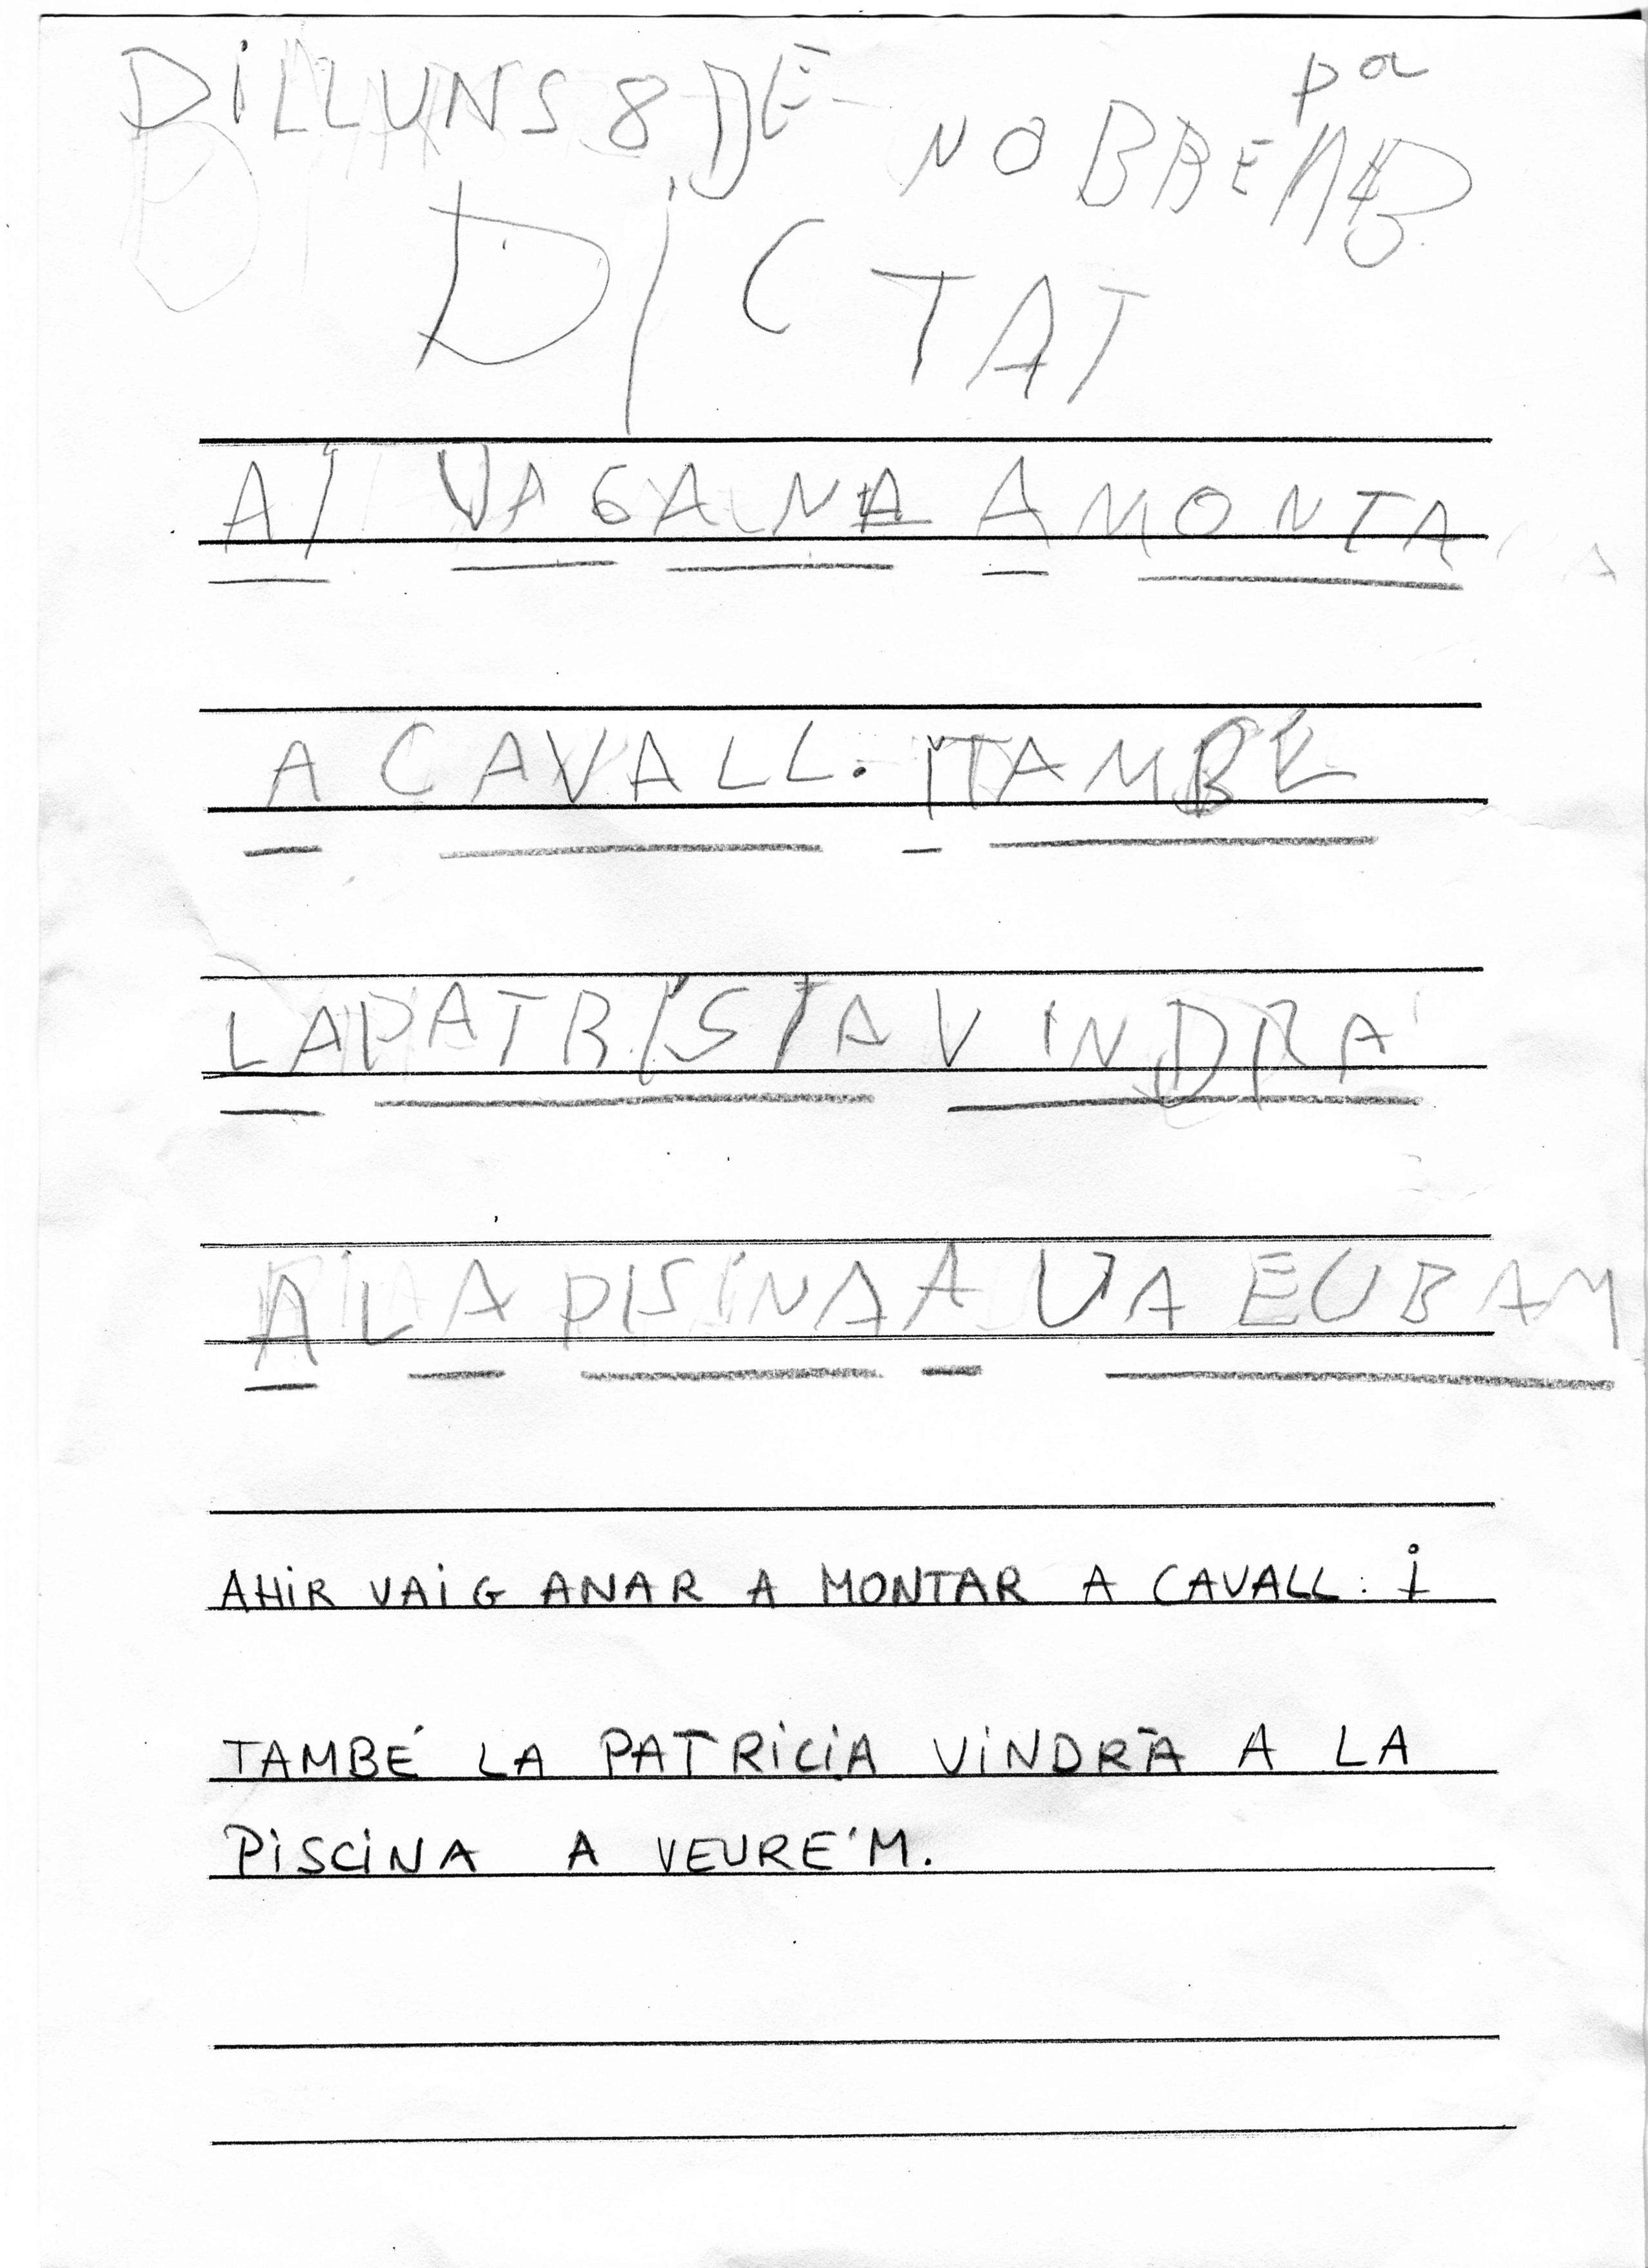
\includegraphics[width=8cm,keepaspectratio]{primaria/img/palmera003108.jpg}}


\end{news}

\noindent\fbox{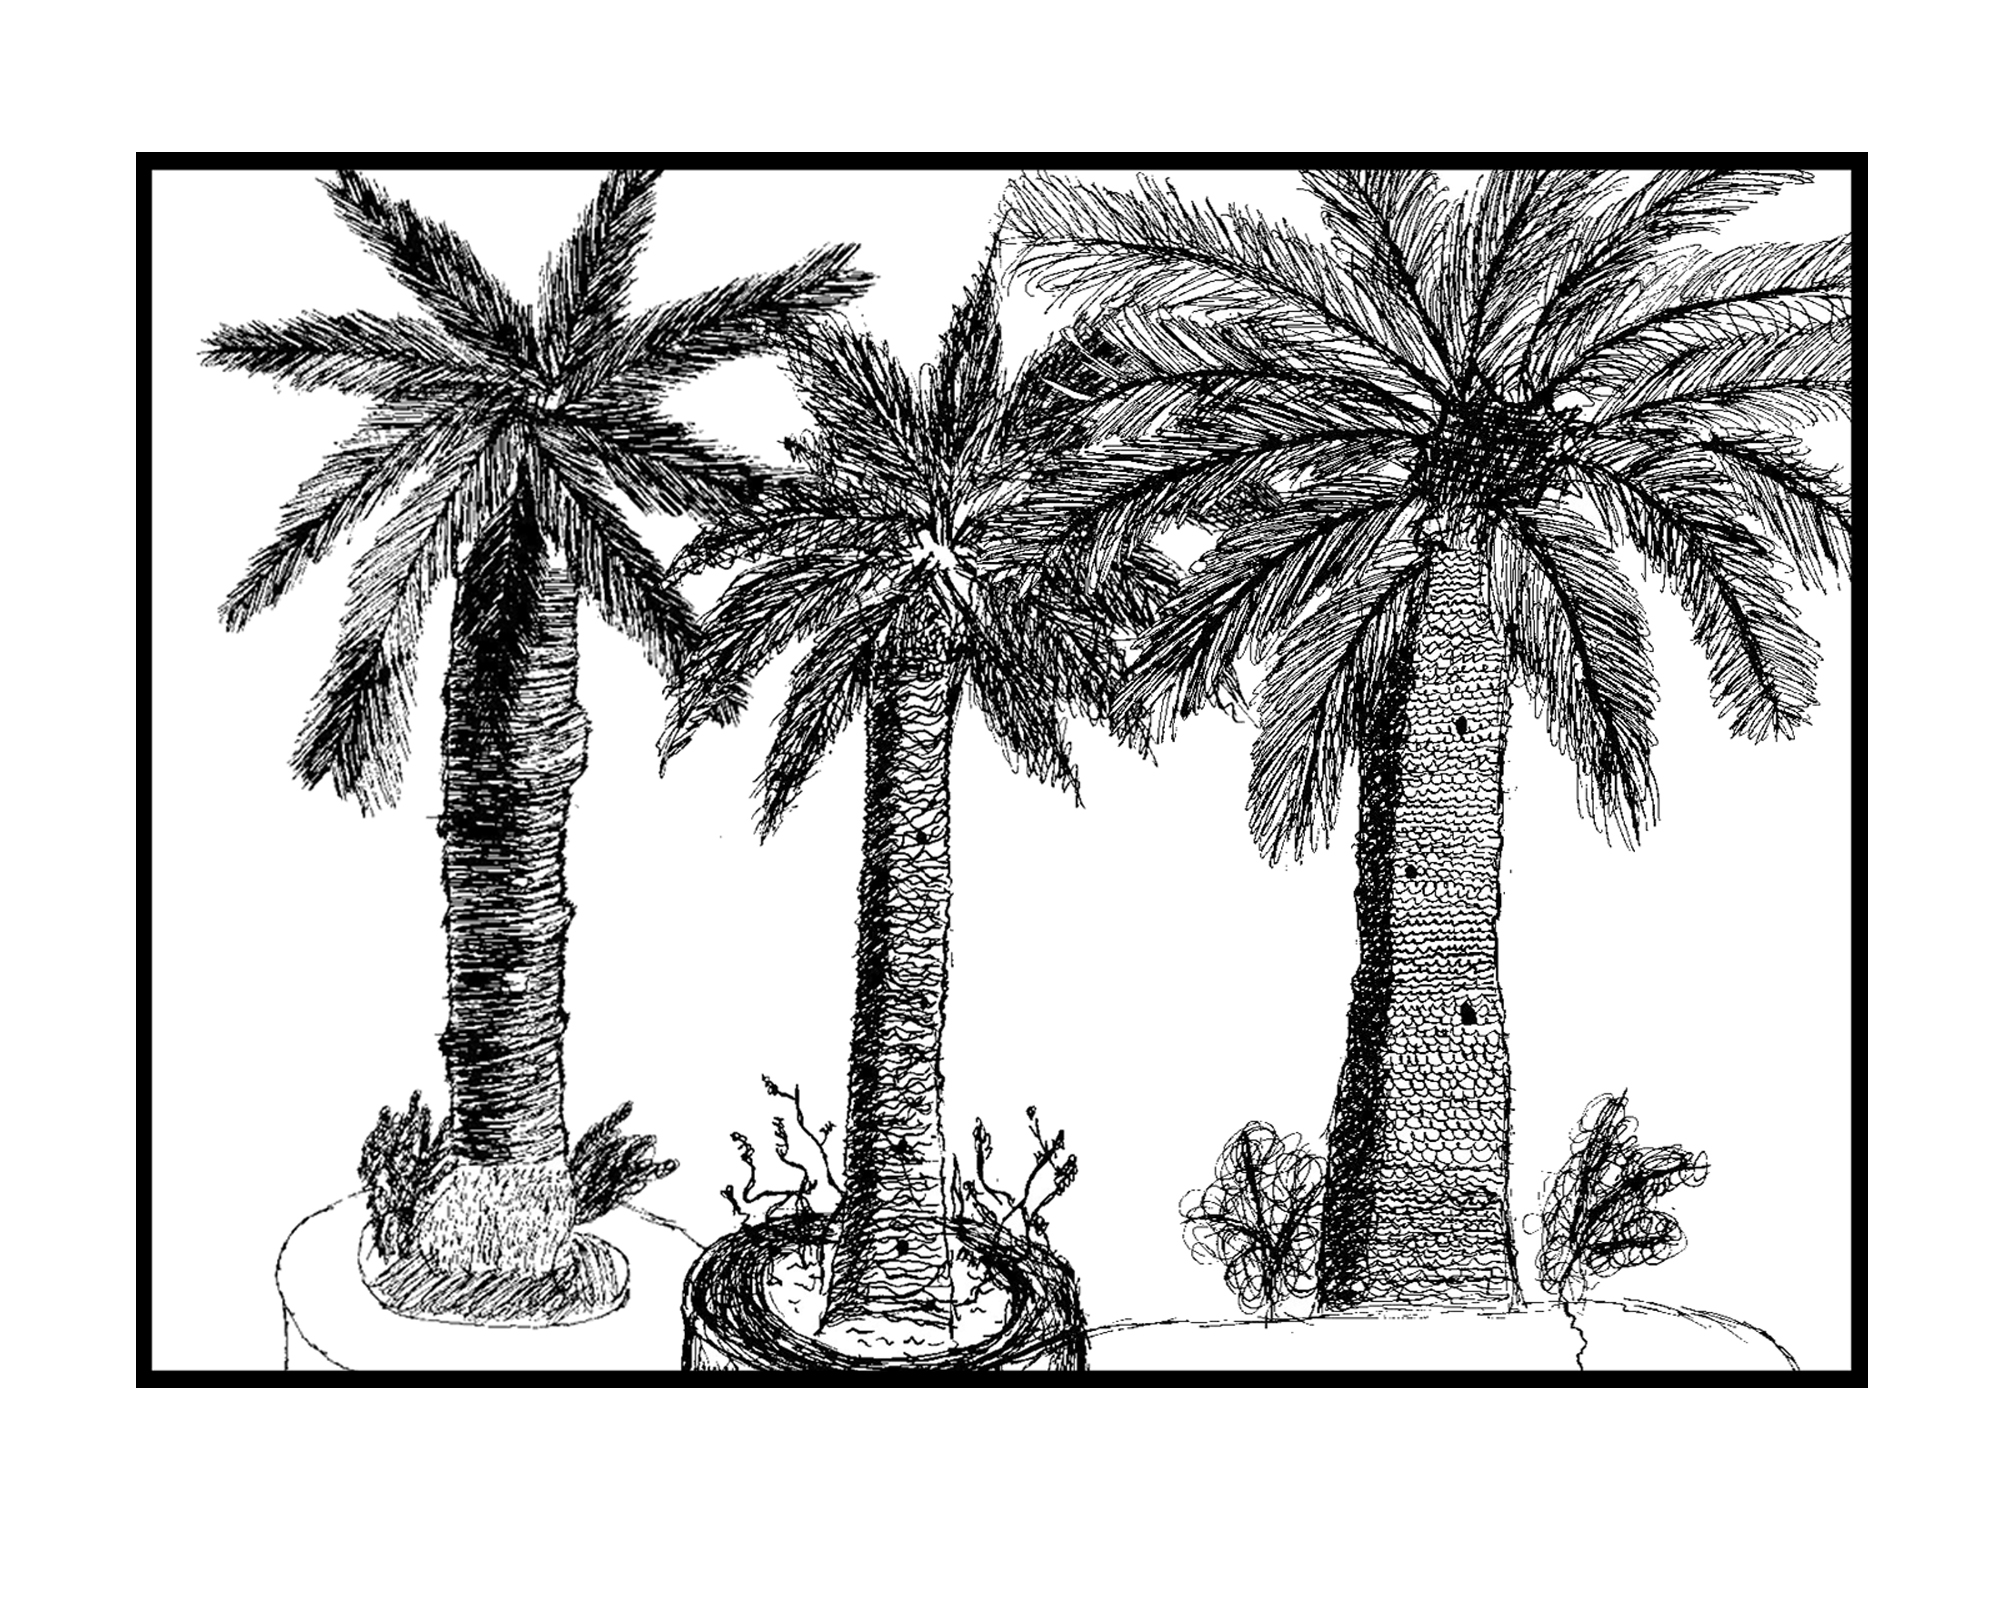
\includegraphics[width=15cm,keepaspectratio]{primaria/img/palmeres_sise.jpg}}
